\section{Score-based ranking và chặn tổng quát hoá}
\label{sec:score-based-ranking-generalization}

Trong phần trước, ta đã giới thiệu các khái niệm cơ bản của bài toán ranking như hàm điểm, quan hệ ưu tiên theo từng cặp, lỗi xếp hạng và margin. Phần này tập trung vào thiết lập \textit{score-based ranking}. Trong thiết lập này, mô hình học một hàm điểm
\[
    h:\mathcal{X}\rightarrow\mathbb{R},
\]
sau đó sinh ranking bằng cách sắp xếp các đối tượng theo điểm số giảm dần.

Mục tiêu chính của phần này là trình bày chặn tổng quát hoá dựa trên margin cho bài toán ranking. Kết quả này cho thấy nếu một hàm điểm có lỗi margin nhỏ trên tập huấn luyện và lớp giả thuyết không quá phức tạp, thì lỗi xếp hạng trên dữ liệu chưa thấy cũng có thể được kiểm soát. Nói cách khác, score-based ranking không chỉ yêu cầu mô hình xếp đúng các cặp đối tượng, mà còn cần tạo ra khoảng cách điểm đủ lớn để thứ tự dự đoán ổn định hơn.

\subsection{Thiết lập score-based ranking}

Gọi \(\mathcal{X}\) là không gian đầu vào. Trong score-based ranking, ta xét một lớp giả thuyết gồm các hàm điểm:
\[
    \mathcal{H}
    \subseteq
    \{h \mid h:\mathcal{X}\rightarrow\mathbb{R}\}.
\]
Với \(h\in\mathcal{H}\), giá trị \(h(x)\) là điểm số của đối tượng \(x\). Nếu
\[
    h(x')>h(x),
\]
thì mô hình xếp \(x'\) cao hơn \(x\). Vì ranking được sinh ra bằng cách sắp xếp điểm số, mọi thứ tự do hàm điểm tạo ra đều có tính bắc cầu. Đây là ưu điểm về mặt đơn giản hoá mô hình, nhưng cũng là hạn chế nếu quan hệ ưu tiên thật có thể không bắc cầu.

Dữ liệu huấn luyện gồm \(m\) cặp đối tượng có nhãn:
\[
    S =
    \big((x_1,x'_1,y_1),\ldots,(x_m,x'_m,y_m)\big),
    \qquad
    y_i\in\{-1,0,+1\}.
\]
Các cặp \((x_i,x'_i)\) được lấy từ một phân phối chưa biết \(D\) trên \(\mathcal{X}\times\mathcal{X}\). Nhãn được xác định bởi hàm ưu tiên mục tiêu
\[
    f:\mathcal{X}\times\mathcal{X}\rightarrow\{-1,0,+1\}.
\]
Theo quy ước, \(f(x,x')=+1\) nghĩa là \(x'\) được ưu tiên hơn \(x\), \(f(x,x')=-1\) nghĩa là \(x\) được ưu tiên hơn \(x'\), và \(f(x,x')=0\) nghĩa là hai đối tượng ngang nhau hoặc không có đủ thông tin.

Với một cặp có nhãn khác \(0\), hàm điểm \(h\) xếp đúng nếu
\begin{equation}
    f(x,x')\big(h(x')-h(x)\big)>0.
    \label{eq:section3-correct-ranking-condition}
\end{equation}
Nếu biểu thức trên nhỏ hơn hoặc bằng \(0\), mô hình xếp sai hoặc không phân biệt được đúng thứ tự giữa hai đối tượng.

\begin{figure}[H]
    \centering
    \begin{tikzpicture}[>=Stealth, node distance=1.8cm]
        \node[draw, rounded corners, align=center, fill=gray!10, minimum width=3.2cm, minimum height=1cm] (data)
        {Dữ liệu cặp\\ \((x,x',y)\)};
        \node[draw, rounded corners, align=center, fill=gray!10, minimum width=3.2cm, minimum height=1cm, right=of data] (score)
        {Hàm điểm\\ \(h:\mathcal{X}\to\mathbb{R}\)};
        \node[draw, rounded corners, align=center, fill=gray!10, minimum width=3.2cm, minimum height=1cm, right=of score] (rank)
        {Sắp xếp theo\\ điểm số \(h(x)\)};
        \draw[->, thick] (data) -- (score);
        \draw[->, thick] (score) -- (rank);
    \end{tikzpicture}
    \caption{Quy trình tổng quát của score-based ranking: học hàm điểm từ các cặp ưu tiên, sau đó dùng điểm số để sinh ranking toàn cục.}
    \label{fig:section3-score-based-pipeline}
\end{figure}

\subsection{Lỗi tổng quát và lỗi thực nghiệm}

Lỗi tổng quát của hàm điểm \(h\) là xác suất mô hình xếp sai một cặp được lấy ngẫu nhiên từ phân phối \(D\):
\begin{equation}
    R(h)
    =
    \Pr_{(x,x')\sim D}
    \left[
        f(x,x')\neq 0
        \ \wedge\
        f(x,x')\big(h(x')-h(x)\big)\leq 0
    \right].
    \label{eq:section3-generalization-error}
\end{equation}
Đại lượng \(R(h)\) là lỗi thật mà ta quan tâm, vì nó đo chất lượng ranking trên dữ liệu chưa thấy. Tuy nhiên, do phân phối \(D\) và hàm mục tiêu \(f\) không được biết đầy đủ, ta dùng lỗi thực nghiệm trên mẫu huấn luyện:
\begin{equation}
    \widehat{R}(h)
    =
    \frac{1}{m}
    \sum_{i=1}^{m}
    \mathbf{1}
    \left[
        y_i\neq 0
        \ \wedge\
        y_i\big(h(x'_i)-h(x_i)\big)\leq 0
    \right].
    \label{eq:section3-empirical-error}
\end{equation}

Để đơn giản hoá phân tích lý thuyết, phần này thường giả sử nhãn chỉ thuộc \(\{-1,+1\}\), tức là mỗi cặp đều có một quan hệ ưu tiên rõ ràng. Khi đó, điều kiện \(y_i\neq 0\) có thể được bỏ đi trong công thức lỗi thực nghiệm.

\subsection{Margin loss cho ranking}

Trong ranking, việc một cặp được xếp đúng chưa hẳn đã đủ. Ta còn muốn mô hình xếp đúng với một khoảng cách điểm đủ lớn. Với một cặp huấn luyện \((x_i,x'_i,y_i)\), margin theo cặp được định nghĩa là:
\begin{equation}
    M_i(h)
    =
    y_i\big(h(x'_i)-h(x_i)\big).
    \label{eq:section3-pairwise-margin}
\end{equation}
Nếu \(M_i(h)>0\), cặp thứ \(i\) được xếp đúng. Nếu \(M_i(h)\leq 0\), cặp đó bị xếp sai. Với một tham số \(\rho>0\), ta định nghĩa hàm mất mát margin:
\begin{equation}
    \Phi_{\rho}(u)
    =
    \begin{cases}
        1, & u\leq 0,\\[0.15cm]
        1-\dfrac{u}{\rho}, & 0<u<\rho,\\[0.25cm]
        0, & u\geq \rho.
    \end{cases}
    \label{eq:section3-margin-loss-function}
\end{equation}

\begin{figure}[H]
    \centering
    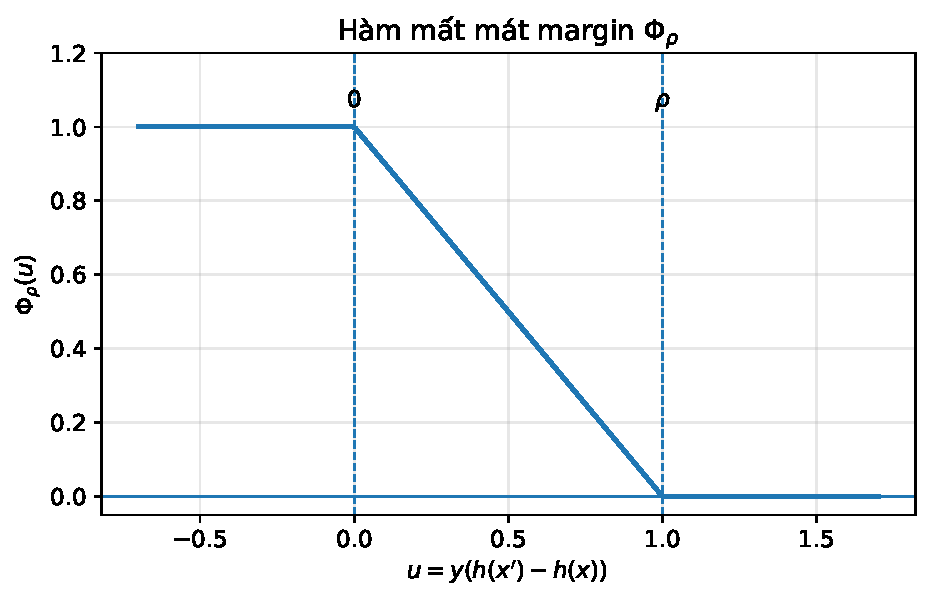
\includegraphics[width=0.82\textwidth]{figures/sec3_margin_loss_phi.pdf}
    \caption{Hàm mất mát margin \(\Phi_{\rho}\). Khi \(u\leq 0\), cặp bị xếp sai hoặc hoà nên bị phạt tối đa. Khi \(0<u<\rho\), cặp đã đúng chiều nhưng margin chưa đủ lớn nên vẫn bị phạt tuyến tính. Khi \(u\geq\rho\), cặp được xem là đúng với độ tin cậy đủ lớn và không bị phạt.}
    \label{fig:section3-margin-loss-phi}
\end{figure}

Hình~\ref{fig:section3-margin-loss-phi} cho thấy vai trò của tham số \(\rho\). Tham số này đặt ra một ngưỡng an toàn cho hiệu điểm giữa hai đối tượng. Nếu margin chỉ vừa lớn hơn \(0\), mô hình tuy xếp đúng nhưng vẫn thiếu chắc chắn; nếu margin vượt qua \(\rho\), mô hình được xem là đã phân biệt cặp đó đủ rõ.

Lỗi margin thực nghiệm được định nghĩa bởi:
\begin{equation}
    \widehat{R}_{\rho}(h)
    =
    \frac{1}{m}
    \sum_{i=1}^{m}
    \Phi_{\rho}
    \left(
        y_i\big(h(x'_i)-h(x_i)\big)
    \right).
    \label{eq:section3-empirical-margin-loss}
\end{equation}
Vì
\[
    \mathbf{1}[u\leq 0]\leq \Phi_{\rho}(u),
\]
nên lỗi thực nghiệm dạng chỉ thị luôn được chặn trên bởi lỗi margin:
\[
    \widehat{R}(h)\leq \widehat{R}_{\rho}(h).
\]
Điều này cho phép ta phân tích ranking thông qua một hàm mất mát mềm hơn và thuận tiện hơn cho việc xây dựng chặn tổng quát hoá.

\subsection{Rademacher complexity}

Để đo độ phức tạp của lớp giả thuyết \(\mathcal{H}\), ta sử dụng Rademacher complexity. Trực giác, Rademacher complexity đo khả năng một lớp hàm có thể khớp với nhiễu ngẫu nhiên. Một lớp hàm có độ phức tạp cao thường dễ overfit hơn.

Với một mẫu \(S=(z_1,\ldots,z_m)\), empirical Rademacher complexity của một lớp hàm \(\mathcal{G}\) được định nghĩa là:
\begin{equation}
    \widehat{\mathfrak{R}}_{S}(\mathcal{G})
    =
    \mathbb{E}_{\sigma}
    \left[
        \sup_{g\in\mathcal{G}}
        \frac{1}{m}
        \sum_{i=1}^{m}
        \sigma_i g(z_i)
    \right],
    \label{eq:section3-empirical-rademacher}
\end{equation}
trong đó \(\sigma_1,\ldots,\sigma_m\) là các biến Rademacher độc lập, nhận giá trị \(+1\) hoặc \(-1\) với xác suất bằng nhau.

Trong bài toán ranking, mỗi mẫu là một cặp \((x_i,x'_i)\). Ta ký hiệu \(D_1\) là phân phối biên của phần tử thứ nhất \(x\), và \(D_2\) là phân phối biên của phần tử thứ hai \(x'\). Tương ứng, ta xét hai đại lượng:
\[
    \mathfrak{R}^{D_1}_m(\mathcal{H}),
    \qquad
    \mathfrak{R}^{D_2}_m(\mathcal{H}).
\]
Hai đại lượng này xuất hiện trong chặn tổng quát hoá vì hàm điểm được đánh giá trên cả hai phần tử của mỗi cặp.

\subsection{Định lý chặn margin cho ranking}

Ta phát biểu kết quả chặn tổng quát hoá chính cho score-based ranking.

\paragraph{Định lý 3.1.}
Cho \(\mathcal{H}\) là một lớp các hàm thực trên \(\mathcal{X}\). Cố định \(\rho>0\). Khi đó, với mọi \(\delta>0\), với xác suất ít nhất \(1-\delta\) theo việc chọn mẫu \(S\) kích thước \(m\), bất đẳng thức sau đúng đồng thời với mọi \(h\in\mathcal{H}\):
\begin{equation}
    R(h)
    \leq
    \widehat{R}_{\rho}(h)
    +
    \frac{2}{\rho}
    \left(
        \mathfrak{R}^{D_1}_m(\mathcal{H})
        +
        \mathfrak{R}^{D_2}_m(\mathcal{H})
    \right)
    +
    \sqrt{
        \frac{\log(1/\delta)}{2m}
    }.
    \label{eq:section3-margin-bound-expected}
\end{equation}

Ngoài ra, ta cũng có dạng chặn theo empirical Rademacher complexity:
\begin{equation}
    R(h)
    \leq
    \widehat{R}_{\rho}(h)
    +
    \frac{2}{\rho}
    \left(
        \widehat{\mathfrak{R}}_{S_1}(\mathcal{H})
        +
        \widehat{\mathfrak{R}}_{S_2}(\mathcal{H})
    \right)
    +
    3
    \sqrt{
        \frac{\log(2/\delta)}{2m}
    }.
    \label{eq:section3-margin-bound-empirical}
\end{equation}

\begin{figure}[H]
    \centering
    \begin{tikzpicture}[>=Stealth, node distance=0.9cm]
        \node[draw, rounded corners, fill=gray!10, align=center, minimum width=3.3cm, minimum height=1.2cm] (train)
        {\(\widehat{R}_{\rho}(h)\)\\ lỗi margin thực nghiệm};
        \node[draw, rounded corners, fill=gray!10, align=center, minimum width=3.8cm, minimum height=1.2cm, right=of train] (complex)
        {\(\dfrac{2}{\rho}(\mathfrak{R}^{D_1}_m+\mathfrak{R}^{D_2}_m)\)\\ độ phức tạp mô hình};
        \node[draw, rounded corners, fill=gray!10, align=center, minimum width=3.3cm, minimum height=1.2cm, right=of complex] (conf)
        {\(\sqrt{\dfrac{\log(1/\delta)}{2m}}\)\\ độ tin cậy};
        \node[draw, rounded corners, fill=gray!20, align=center, minimum width=3.3cm, minimum height=1.2cm, below=1.4cm of complex] (gen)
        {\(R(h)\)\\ lỗi tổng quát};
        \draw[->, thick] (train.south) -- (gen.north west);
        \draw[->, thick] (complex.south) -- (gen.north);
        \draw[->, thick] (conf.south) -- (gen.north east);
    \end{tikzpicture}
    \caption{Ba thành phần trong chặn tổng quát hoá: lỗi trên tập huấn luyện, độ phức tạp của lớp giả thuyết và sai số do lấy mẫu hữu hạn.}
    \label{fig:section3-margin-bound-components}
\end{figure}

Chặn trên gồm ba thành phần. Thành phần thứ nhất là lỗi margin thực nghiệm \(\widehat{R}_{\rho}(h)\). Thành phần thứ hai phụ thuộc vào độ phức tạp của lớp giả thuyết \(\mathcal{H}\). Thành phần thứ ba phụ thuộc vào kích thước mẫu \(m\) và mức tin cậy \(\delta\).

Định lý cho thấy để lỗi tổng quát \(R(h)\) nhỏ, ta cần đồng thời giảm lỗi margin thực nghiệm và kiểm soát độ phức tạp của lớp giả thuyết. Tham số \(\rho\) tạo ra một sự đánh đổi: nếu \(\rho\) lớn, yêu cầu margin nghiêm ngặt hơn nên lỗi margin thực nghiệm có thể tăng; nếu \(\rho\) nhỏ, hệ số \(1/\rho\) trong thành phần độ phức tạp lại tăng.

\subsection{Chứng minh Định lý 3.1}

Đặt \(z=((x,x'),y)\) và định nghĩa lớp hàm margin theo cặp:
\[
    \mathcal{H}_{\Delta}
    =
    \left\{
        ((x,x'),y)
        \mapsto
        y\big(h(x')-h(x)\big)
        \mid
        h\in\mathcal{H}
    \right\}.
\]
Với mỗi \(h\in\mathcal{H}\), nếu một cặp bị xếp sai thì
\[
    y(h(x')-h(x))\leq 0.
\]
Do \(\mathbf{1}[u\leq 0]\leq \Phi_{\rho}(u)\), ta có
\[
    R(h)
    =
    \mathbb{E}_{z}
    \mathbf{1}
    \left[
        y(h(x')-h(x))\leq 0
    \right]
    \leq
    \mathbb{E}_{z}
    \Phi_{\rho}
    \left(
        y(h(x')-h(x))
    \right).
\]
Vì vậy, chỉ cần chặn sai khác giữa kỳ vọng thật và trung bình thực nghiệm của lớp hàm sau:
\[
    \Phi_{\rho}\circ\mathcal{H}_{\Delta}
    =
    \left\{
        ((x,x'),y)
        \mapsto
        \Phi_{\rho}
        \left(
            y\big(h(x')-h(x)\big)
        \right)
        \mid
        h\in\mathcal{H}
    \right\}.
\]

Lớp \(\Phi_{\rho}\circ\mathcal{H}_{\Delta}\) nhận giá trị trong \([0,1]\). Áp dụng chặn tổng quát hoá bằng Rademacher complexity cho lớp hàm bị chặn, với xác suất ít nhất \(1-\delta\), đồng thời với mọi \(h\in\mathcal{H}\):
\[
    \mathbb{E}_{z}
    \Phi_{\rho}
    \left(
        y(h(x')-h(x))
    \right)
    \leq
    \widehat{R}_{\rho}(h)
    +
    2
    \mathfrak{R}_m
    \left(
        \Phi_{\rho}\circ\mathcal{H}_{\Delta}
    \right)
    +
    \sqrt{
        \frac{\log(1/\delta)}{2m}
    }.
\]
Kết hợp với bất đẳng thức \(R(h)\leq \mathbb{E}_{z}\Phi_{\rho}(y(h(x')-h(x)))\), ta được bước chặn đầu tiên.

Tiếp theo, ta chặn độ phức tạp của lớp \(\Phi_{\rho}\circ\mathcal{H}_{\Delta}\). Hàm \(\Phi_{\rho}\) là \(1/\rho\)-Lipschitz. Khi áp dụng định lý contraction, việc cộng một hằng số vào hàm mất mát không làm thay đổi Rademacher complexity vì
\[
    \mathbb{E}_{\sigma}
    \left[
        \frac{1}{m}
        \sum_{i=1}^{m}
        \sigma_i c
    \right]
    =
    0.
\]
Do đó:
\[
    \mathfrak{R}_m
    \left(
        \Phi_{\rho}\circ\mathcal{H}_{\Delta}
    \right)
    \leq
    \frac{1}{\rho}
    \mathfrak{R}_m(\mathcal{H}_{\Delta}).
\]

Ta còn cần chặn \(\mathfrak{R}_m(\mathcal{H}_{\Delta})\) theo độ phức tạp của \(\mathcal{H}\). Với một mẫu \(S=\{((x_i,x'_i),y_i)\}_{i=1}^{m}\), ta có:
\[
\begin{aligned}
    \widehat{\mathfrak{R}}_{S}(\mathcal{H}_{\Delta})
    &=
    \mathbb{E}_{\sigma}
    \left[
        \sup_{h\in\mathcal{H}}
        \frac{1}{m}
        \sum_{i=1}^{m}
        \sigma_i y_i
        \big(h(x'_i)-h(x_i)\big)
    \right] \\
    &\leq
    \mathbb{E}_{\sigma}
    \left[
        \sup_{h\in\mathcal{H}}
        \frac{1}{m}
        \sum_{i=1}^{m}
        \sigma_i y_i h(x'_i)
    \right]
    +
    \mathbb{E}_{\sigma}
    \left[
        \sup_{h\in\mathcal{H}}
        \frac{1}{m}
        \sum_{i=1}^{m}
        (-\sigma_i y_i) h(x_i)
    \right].
\end{aligned}
\]
Vì \(y_i\in\{-1,+1\}\), các biến \(\sigma_i y_i\) và \(-\sigma_i y_i\) vẫn là các biến Rademacher độc lập. Lấy kỳ vọng theo mẫu, hạng thứ nhất trở thành \(\mathfrak{R}^{D_2}_m(\mathcal{H})\), còn hạng thứ hai trở thành \(\mathfrak{R}^{D_1}_m(\mathcal{H})\). Suy ra:
\[
    \mathfrak{R}_m(\mathcal{H}_{\Delta})
    \leq
    \mathfrak{R}^{D_1}_m(\mathcal{H})
    +
    \mathfrak{R}^{D_2}_m(\mathcal{H}).
\]
Thay hai chặn trên vào bất đẳng thức tổng quát hoá, ta thu được:
\[
    R(h)
    \leq
    \widehat{R}_{\rho}(h)
    +
    \frac{2}{\rho}
    \left(
        \mathfrak{R}^{D_1}_m(\mathcal{H})
        +
        \mathfrak{R}^{D_2}_m(\mathcal{H})
    \right)
    +
    \sqrt{
        \frac{\log(1/\delta)}{2m}
    },
\]
đúng đồng thời với mọi \(h\in\mathcal{H}\). Đây chính là dạng chặn theo Rademacher complexity kỳ vọng.

Để thu được dạng empirical Rademacher complexity, ta dùng chặn chuẩn liên hệ giữa độ phức tạp kỳ vọng và độ phức tạp thực nghiệm. Cụ thể, với xác suất cao, mỗi đại lượng \(\mathfrak{R}^{D_j}_m(\mathcal{H})\) có thể được thay bởi \(\widehat{\mathfrak{R}}_{S_j}(\mathcal{H})\) cộng thêm một sai số lấy mẫu bậc \(\sqrt{\log(1/\delta)/m}\). Áp dụng bất đẳng thức này cho hai phân phối biên \(D_1,D_2\) và dùng union bound cho các biến cố xác suất, các hạng sai số được gom lại thành
\[
    3
    \sqrt{
        \frac{\log(2/\delta)}{2m}
    }.
\]
Do đó, với xác suất ít nhất \(1-\delta\), đồng thời với mọi \(h\in\mathcal{H}\):
\[
    R(h)
    \leq
    \widehat{R}_{\rho}(h)
    +
    \frac{2}{\rho}
    \left(
        \widehat{\mathfrak{R}}_{S_1}(\mathcal{H})
        +
        \widehat{\mathfrak{R}}_{S_2}(\mathcal{H})
    \right)
    +
    3
    \sqrt{
        \frac{\log(2/\delta)}{2m}
    }.
\]
Vậy cả hai bất đẳng thức trong Định lý 3.1 đều được chứng minh.

\subsection{[MỞ RỘNG] Giải thích bước Lipschitz của \texorpdfstring{\(\Phi_{\rho}\)}{Phi rho}}

Từ định nghĩa của \(\Phi_{\rho}\), ta thấy hàm này là hằng số trên \((-\infty,0]\), giảm tuyến tính trên \((0,\rho)\), và lại là hằng số trên \([\rho,+\infty)\). Trên đoạn giữa, độ dốc của hàm là
\[
    -\frac{1}{\rho}.
\]
Do đó, với mọi \(u,v\in\mathbb{R}\), ta có:
\[
    |\Phi_{\rho}(u)-\Phi_{\rho}(v)|
    \leq
    \frac{1}{\rho}|u-v|.
\]
Vì vậy, \(\Phi_{\rho}\) là hàm \(1/\rho\)-Lipschitz. Đây là lý do trong bước contraction, Rademacher complexity của lớp sau khi ghép với \(\Phi_{\rho}\) được nhân với hệ số \(1/\rho\). Trực quan từ Hình~\ref{fig:section3-margin-loss-phi}, độ dốc lớn nhất về trị tuyệt đối của đồ thị chính là \(1/\rho\).

\subsection{Hệ quả cho lớp hàm kernel}

Một hệ quả quan trọng của Định lý 3.1 là chặn tổng quát hoá cho lớp hàm kernel. Giả sử \(K:\mathcal{X}\times\mathcal{X}\rightarrow\mathbb{R}\) là một kernel xác định dương, \(\Phi:\mathcal{X}\rightarrow\mathcal{F}\) là ánh xạ đặc trưng tương ứng, và xét lớp giả thuyết:
\[
    \mathcal{H}
    =
    \left\{
        x\mapsto w\cdot \Phi(x)
        \mid
        \|w\|_{\mathcal{F}}\leq \Lambda
    \right\}.
\]
Đặt
\[
    r=\sup_{x\in\mathcal{X}}K(x,x).
\]
Khi đó, với xác suất ít nhất \(1-\delta\), với mọi \(h\in\mathcal{H}\), ta có:
\begin{equation}
    R(h)
    \leq
    \widehat{R}_{\rho}(h)
    +
    4
    \sqrt{
        \frac{r^2\Lambda^2}{\rho^2 m}
    }
    +
    \sqrt{
        \frac{\log(1/\delta)}{2m}
    }.
    \label{eq:section3-kernel-margin-bound}
\end{equation}

Chặn này đáng chú ý vì nó không phụ thuộc trực tiếp vào số chiều của không gian đặc trưng \(\mathcal{F}\). Thay vào đó, nó phụ thuộc vào margin \(\rho\), kích thước mẫu \(m\), cận \(r\) của kernel và chuẩn của vector trọng số thông qua \(\Lambda\).

\subsection{[MỞ RỘNG] Phân tích độ phức tạp của score-based ranking}

Ranking theo từng cặp có thể tốn kém vì số lượng cặp tăng nhanh theo số đối tượng. Nếu có \(n\) đối tượng và xét tất cả các cặp không lặp, số lượng cặp là:
\begin{equation}
    |\mathcal{P}|
    =
    \binom{n}{2}
    =
    \frac{n(n-1)}{2}
    =
    O(n^2).
    \label{eq:section3-number-of-pairs}
\end{equation}

\begin{figure}[H]
    \centering
    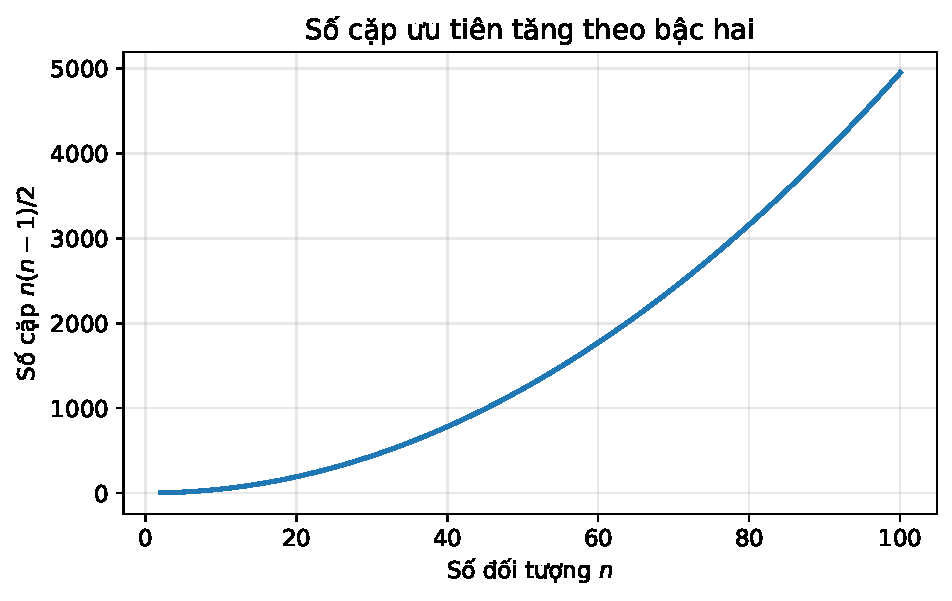
\includegraphics[width=0.82\textwidth]{figures/sec3_pair_count_complexity.pdf}
    \caption{Số cặp ưu tiên tăng theo bậc hai khi số đối tượng \(n\) tăng. Với \(n=100\), nếu xét toàn bộ các cặp không lặp thì có \(\binom{100}{2}=4950\) cặp.}
    \label{fig:section3-pair-count-complexity}
\end{figure}

Hình~\ref{fig:section3-pair-count-complexity} minh hoạ vì sao pairwise ranking có thể nhanh chóng trở nên tốn kém khi \(n\) lớn. Chỉ cần tăng số đối tượng, số cặp cần xét tăng nhanh hơn nhiều so với \(n\). Đây là lý do các hệ thống ranking thực tế thường không huấn luyện trên toàn bộ mọi cặp có thể, mà dùng lấy mẫu cặp, mini-batch hoặc các kỹ thuật tối ưu chuyên biệt.

Với mô hình tuyến tính \(h_w(x)=w^\top x\), chi phí tính điểm cho \(n\) đối tượng là \(O(nd)\), và chi phí sắp xếp để tạo ranking là \(O(n\log n)\). Do đó, chi phí suy luận là:
\[
    O(nd+n\log n).
\]
Nếu huấn luyện trực tiếp trên toàn bộ các cặp, mỗi cặp cần tính hiệu điểm
\[
    h_w(x_j)-h_w(x_i)=w^\top(x_j-x_i),
\]
có chi phí \(O(d)\). Vì vậy, chi phí cho một epoch huấn luyện là:
\[
    O(n^2d).
\]

\begin{table}[H]
    \centering
    \begin{tabular}{lll}
        \toprule
        \textbf{Bước xử lý} & \textbf{Chi phí} & \textbf{Ý nghĩa} \\
        \midrule
        Tính điểm cho \(n\) đối tượng & \(O(nd)\) & Tính \(h_w(x)=w^\top x\) \\
        Sắp xếp để tạo ranking & \(O(n\log n)\) & Xếp đối tượng theo điểm giảm dần \\
        Tạo toàn bộ cặp & \(O(n^2)\) & Số cặp tăng theo \(\binom{n}{2}\) \\
        Một epoch pairwise training & \(O(n^2d)\) & Tính loss/gradient trên mọi cặp \\
        \bottomrule
    \end{tabular}
    \caption{Tóm tắt độ phức tạp của score-based pairwise ranking với mô hình tuyến tính.}
    \label{tab:section3-complexity-summary}
\end{table}

\subsection{Ví dụ minh hoạ về margin}

Xét ba tài liệu \(d_1,d_2,d_3\) với thứ tự đúng:
\[
    d_1 \succ d_2 \succ d_3.
\]
Giả sử mô hình dự đoán điểm:
\[
    h(d_1)=2.0,
    \qquad
    h(d_2)=1.2,
    \qquad
    h(d_3)=1.1.
\]

\begin{figure}[H]
    \centering
    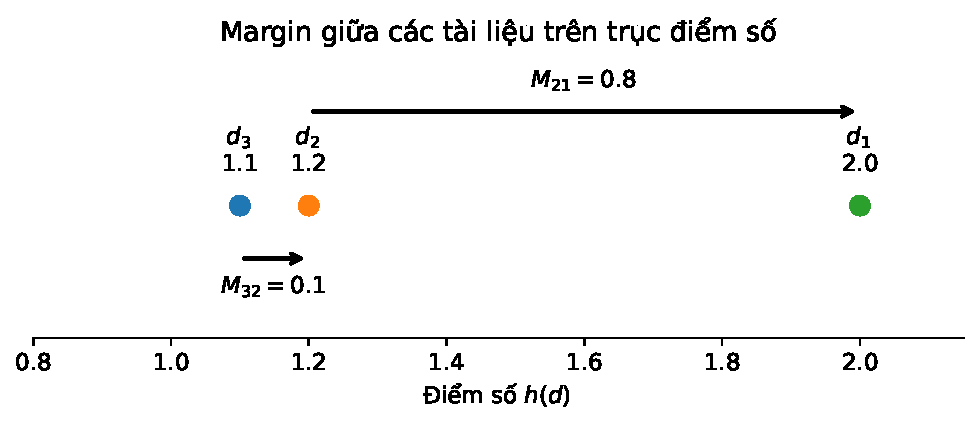
\includegraphics[width=0.86\textwidth]{figures/sec3_margin_on_score_axis.pdf}
    \caption{Minh hoạ margin giữa các tài liệu trên trục điểm số. Cặp \((d_2,d_1)\) có margin lớn hơn, trong khi cặp \((d_3,d_2)\) có margin nhỏ nên kém chắc chắn hơn dù vẫn được xếp đúng.}
    \label{fig:section3-margin-on-score-axis}
\end{figure}

Với cặp \((d_2,d_1)\), margin là:
\[
    M_{21}(h)
    =
    h(d_1)-h(d_2)
    =
    0.8.
\]
Với cặp \((d_3,d_2)\), margin là:
\[
    M_{32}(h)
    =
    h(d_2)-h(d_3)
    =
    0.1.
\]
Cả hai cặp đều được xếp đúng vì margin dương. Tuy nhiên, Hình~\ref{fig:section3-margin-on-score-axis} cho thấy hai trường hợp này không có cùng mức độ chắc chắn. Cặp \((d_2,d_1)\) có khoảng cách điểm lớn, còn cặp \((d_3,d_2)\) chỉ cách nhau \(0.1\), nên dễ bị đảo thứ tự nếu điểm dự đoán có nhiễu nhỏ.

Nếu chọn \(\rho=0.5\), cặp \((d_3,d_2)\) vẫn bị phạt bởi margin loss vì margin chỉ bằng \(0.1\), nhỏ hơn \(\rho\):
\[
    \Phi_{0.5}(0.1)
    =
    1-\frac{0.1}{0.5}
    =
    0.8.
\]
Ví dụ này cho thấy margin loss không chỉ quan tâm đến việc xếp đúng hay sai, mà còn quan tâm đến mức độ chắc chắn của thứ tự được dự đoán.

\subsection{Tóm tắt}

Phần này đã trình bày thiết lập score-based ranking, trong đó mô hình học một hàm điểm \(h:\mathcal{X}\rightarrow\mathbb{R}\) và dùng hàm này để sinh thứ tự xếp hạng. Ta đã định nghĩa lỗi tổng quát, lỗi thực nghiệm, margin theo cặp và lỗi margin thực nghiệm. Kết quả chính là chặn tổng quát hoá dựa trên Rademacher complexity, cho thấy lỗi ranking có thể được kiểm soát thông qua lỗi margin thực nghiệm và độ phức tạp của lớp giả thuyết.

Các hình minh hoạ trong phần này giúp làm rõ ba ý chính. Thứ nhất, \(\Phi_{\rho}\) là một surrogate loss mềm hơn lỗi chỉ thị và phạt cả các cặp đúng nhưng margin nhỏ. Thứ hai, margin có thể được hiểu trực quan là khoảng cách điểm giữa hai đối tượng trên trục score. Thứ ba, số lượng cặp trong pairwise ranking tăng theo \(O(n^2)\), khiến việc huấn luyện trực tiếp trên toàn bộ cặp trở nên tốn kém với dữ liệu lớn.

Các kết quả trên cũng giải thích vì sao các thuật toán ranking dựa trên margin thường tìm một hàm điểm vừa có lỗi margin nhỏ, vừa có độ phức tạp được kiểm soát. Đây là cơ sở tự nhiên dẫn đến các phương pháp như Ranking SVM ở phần tiếp theo.
